%\documentclass[compress,t,11pt]{beamer}
\documentclass[handout,compress,t,11pt]{beamer}
\usetheme[]{metropolis}           % Use metropolis theme
\usefonttheme{serif}
\definecolor[named]{Gray}{RGB}{111,112,114}
\definecolor[named]{DarkGray}{RGB}{48,48,48}
\definecolor[named]{Cardinal}{RGB}{179,22,34}
\usepackage[T1]{fontenc}
\usepackage[altbullet]{lucidabr}
\usepackage{textcomp}
\usepackage{upquote} % needed to make straight quotes work in listings
\usepackage{listgolang}
\usepackage{mathtools}
\usepackage{comment}
\usepackage{tikz}
\usepackage{tikzsymbols}
 \usetikzlibrary{trees,shapes,plotmarks,arrows,er,automata,petri,topaths,positioning}
\usepackage{pifont}
\usepackage{clrscode}
\usepackage{setspace}
\usepackage{soul}
\usepackage{hyperref}

\setbeamercolor{palette primary}{fg=white,bg=Cardinal}
\setbeamercolor{palette secondary}{fg=white,bg=Gray}
\setbeamercolor{palette tertiary}{fg=white,bg=Cardinal}
\setbeamercolor{palette quaternary}{fg=white,bg=Gray}
\setbeamercolor{palette sidebar primary}{fg=white,bg=Cardinal}
\setbeamercolor{palette sidebar secondary}{fg=white,bg=Gray}
\setbeamercolor*{titlelike}{fg=Cardinal}
\setbeamercolor{structure}{fg=Gray}
\setbeamercolor{title separator}{fg=Cardinal}
\setbeamercolor{alerted text}{fg=Cardinal}
\setbeamercolor{reversed}{fg=Cardinal,bg=black}

\newcommand{\card}[1]{\ensuremath{\left|#1\right|}}
\newcommand{\norm}[1]{\ensuremath{\|#1\|}}

\title[Programming in Go]{\bf Programming in Go\\ Lesson 2: Packages \& Functions}
\author{Matt Holiday} 
\institute[CP]{Cardinal Peak}
\date{23 April 2019} 
%\titlegraphic{\hfill
\includegraphics[width=.25\textwidth,height=.25\textheight]{cp-logo-2x.png}}
\titlegraphic{
\begin{tikzpicture}[overlay, remember picture,scale=0.4]
\node[at=(current page.north east), anchor=north east] (a) {};
\node[below left = 0.1cm and 0.1cm of a] (b)
{
\includegraphics[width=.25\textwidth,height=.25\textheight]{cp-logo-2x.png}};
\node[below left=2.56cm and 2.9cm of b]
{
\includegraphics[width=.1\textwidth]{go-logo.png}};
\end{tikzpicture}}

\setbeamerfont{footline}{series=\bfseries\selectfont}
\setbeamersize{text margin left=12pt,text margin right=12pt}
\linespread{1.0}
\metroset{block=fill}

\hypersetup{
    colorlinks=true,
    linkcolor=Cardinal,
    filecolor=magenta,      
    urlcolor=blue,
}

\begin{document}
\frame{\titlepage} 

%\section{Introduction}
\begin{frame}[fragile]
    \frametitle{Lesson \#2}
    What we'll cover today:
    \begin{itemize}
    \item Homework \#1
    \item Slice gotchas
    \item IDEs
    \item Packages
    \item Functions, parms, \& returns
    \item Scope of variables
    \item Gotchas with \verb|:=|
    \item Closures
    \item Defer
    \end{itemize}
\end{frame}

% =================================================================================

\begin{frame}[fragile]
\frametitle{Homework \#1: First program}
\begin{golang}
package main

import (
    "fmt"
    "io/ioutil"
    "os"
    "strings"
)

func main() {
    var n int

    // don't use range here, you don't want the first arg!

    for i := 1; i < len(os.Args); i++ {
        fn := os.Args[i]
        text, err := ioutil.ReadFile(fn)
\end{golang}
\end{frame}
\begin{frame}[fragile]
\frametitle{Homework \#1: First program}
\begin{golang}
        // handle the case of a bad file name

        if err != nil {
            fmt.Fprintf(os.Stderr, "can't read %s: %s\n",
                        fn, err)
            continue
        }

        // magic happens here
        // we must convert the []byte from ReadFile

        words := strings.Fields(string(text))
        n += len(words)
    }

    fmt.Println(n, "total words")
}
\end{golang}
\end{frame}

\begin{frame}[fragile]
\frametitle{Homework \#1: Second program}
\begin{golang}
func main() {
    m := make(map[string]int)  // can't just use var

    for i := 1; i < len(os.Args); i++ {
        fn := os.Args[i]
        text, err := ioutil.ReadFile(fn)

        if err != nil { /* error handling here */ }

        words := strings.Fields(string(text))

        for _, w := range words {  // ignore keys
            m[w] += 1  // m[w] returns 0 on first access
        }
    }

    fmt.Println(len(m), "unique words")
}
\end{golang}
\end{frame}

\begin{frame}[fragile]
\frametitle{Homework \#1: Results}
{\scriptsize
\begin{verbatim}
## file rich2.txt is taken from Shakespeare, Richard II act 2 scene 1

$ go run counter1.go rich2.txt
2558 total words

$ wc rich2.txt
     372    2558   14102 rich2.txt

$ go run counter2.go rich2.txt
1197 unique words

$ awk '{for (i=1; i<=NF; i++) {print $i}}' rich2.txt|sort|uniq|wc
    1197    1197    7993

$ awk '{for (i=1; i<=NF; i++) {print $i}}' rich2.txt|sort|uniq|head -5
&
'Gainst
'Tis
'gainst
'mongst
\end{verbatim}}
\end{frame}

\begin{frame}[fragile]
\frametitle{``Understanding nil''}
\begin{center}

\includegraphics[width=0.9\textwidth]{new-language-quote.png}
\end{center}
\end{frame}

\section{Slice Gotchas}

\begin{frame}[fragile]
\frametitle{Slice follow-up}
\begin{center}
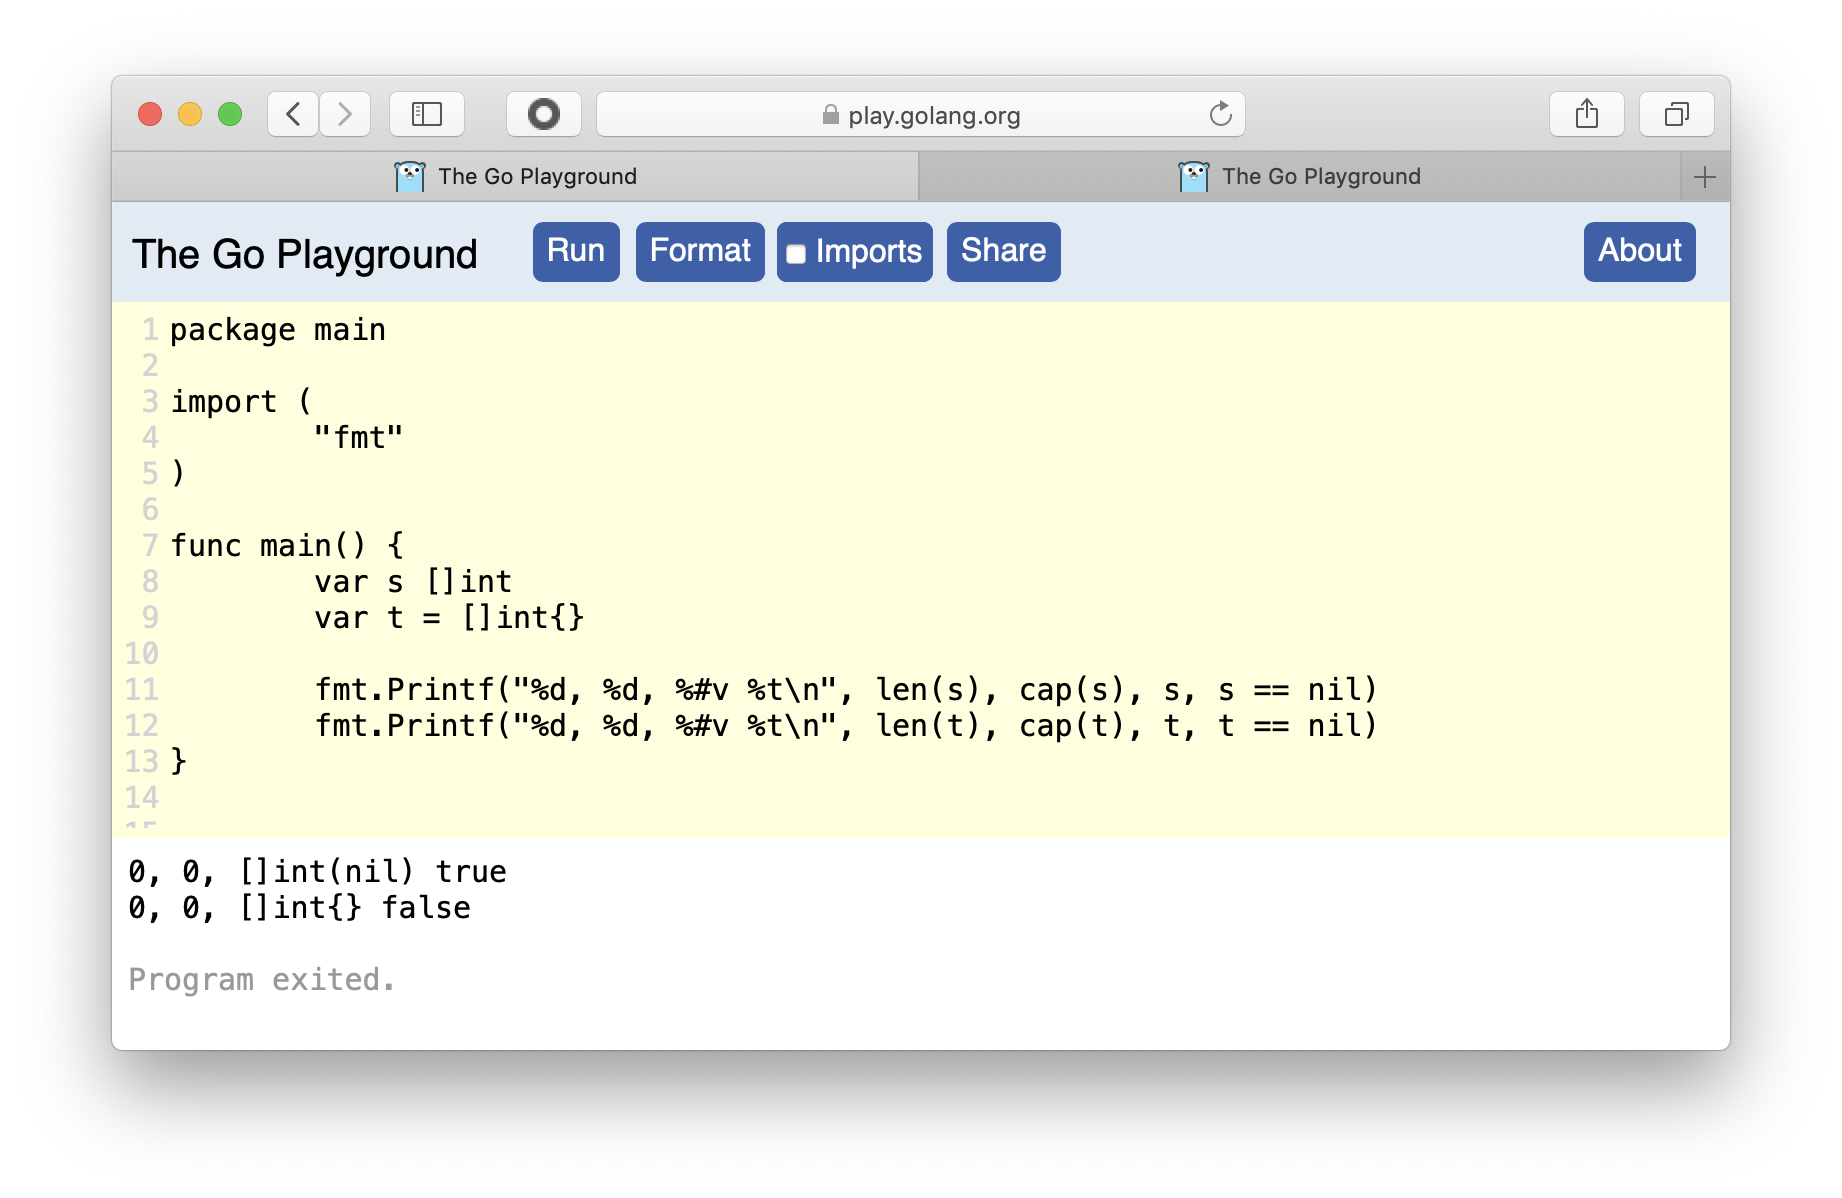
\includegraphics[height=0.9\textheight]{slice-declarations.png}
\end{center}
\end{frame}

\begin{frame}[fragile]
\frametitle{Slice follow-up}
\begin{center}
\vspace{3\baselineskip}
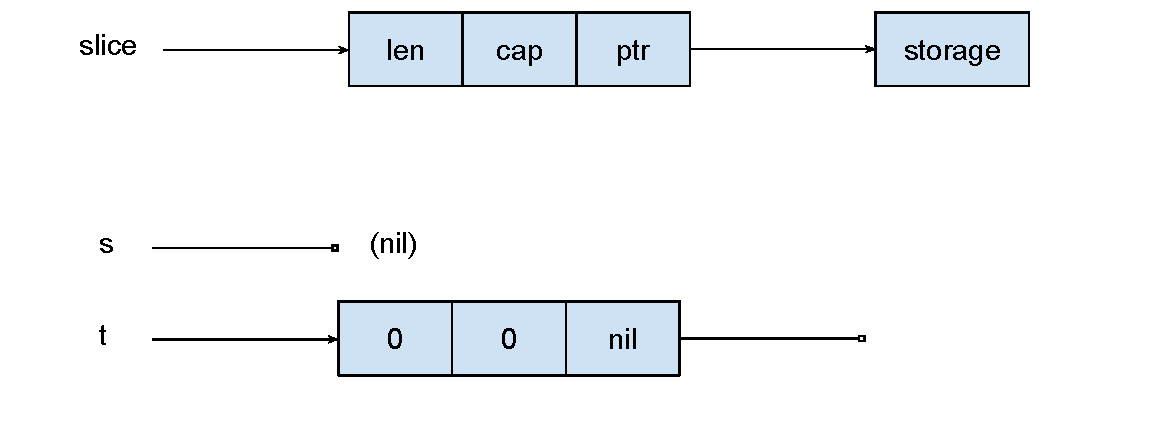
\includegraphics[width=0.9\textwidth]{slice-picture.pdf}
\end{center}
\end{frame}

\begin{frame}[fragile]
    \frametitle{Ugly \#1: Slice length vs capacity}
\begin{golang}
// let's make an array of 3 items

a := [3]int{1, 2, 3}

b := a[0:1]          // b is a slice of a's first item

fmt.Println(b)       // prints [1]

c := b[0:2]          // WTF? but the array has 3 entries

fmt.Println(c)       // prints [1 2]

fmt.Println(len(b))  // prints 1
fmt.Println(cap(b))  // prints 3

b := a[0:1:1]        // this is what you probably meant
\end{golang}
\end{frame}

\begin{frame}[fragile]
    \frametitle{Ugly \#2: Slice mutating underlying array}
\begin{golang}
a := [3]int{1, 2, 3}
b := a[0:1]; c := b[0:2]

b = append(b, 4)      // grows b, mutates a
fmt.Println("a=",a)   // a= [1 4 3]
fmt.Println("b=",b)   // b= [1 4]

c = append(c, 5)      // grows c, mutates a
fmt.Println("a=",a)   // a= [1 4 5]
fmt.Println("c=",c)   // c= [1 4 5]

c = append(c, 6)      // forces allocation!
fmt.Println("a=",a)   // a= [1 4 5]
fmt.Println("c=",c)   // c= [1 4 5 6]

c[0] = 9              // mutates a different array!
fmt.Println("a=",a)   // a= [1 4 5]
fmt.Println("c=",c)   // c= [9 4 5 6]
\end{golang}
\end{frame}


% =================================================================================

\section{Development Environments}

\begin{frame}[fragile]
    \frametitle{Vim}
    \begin{center}
    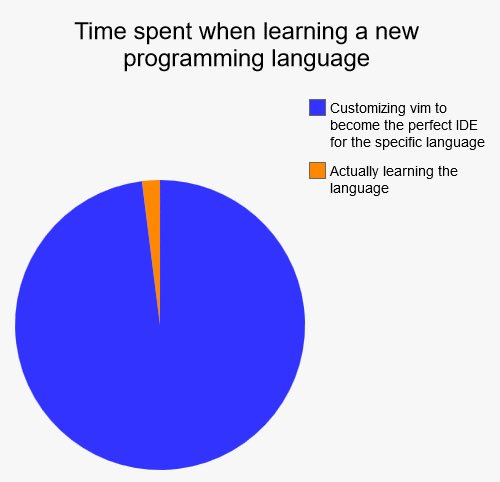
\includegraphics[width=0.5\textwidth]{vim-ide-joke.jpg}
    \end{center}
    \href{https://tpaschalis.github.io/vim-go-setup/}{Vim setup example}
\end{frame}


\begin{frame}[fragile]
    \frametitle{Jetbrains GoLand IDE}
    \begin{center}
    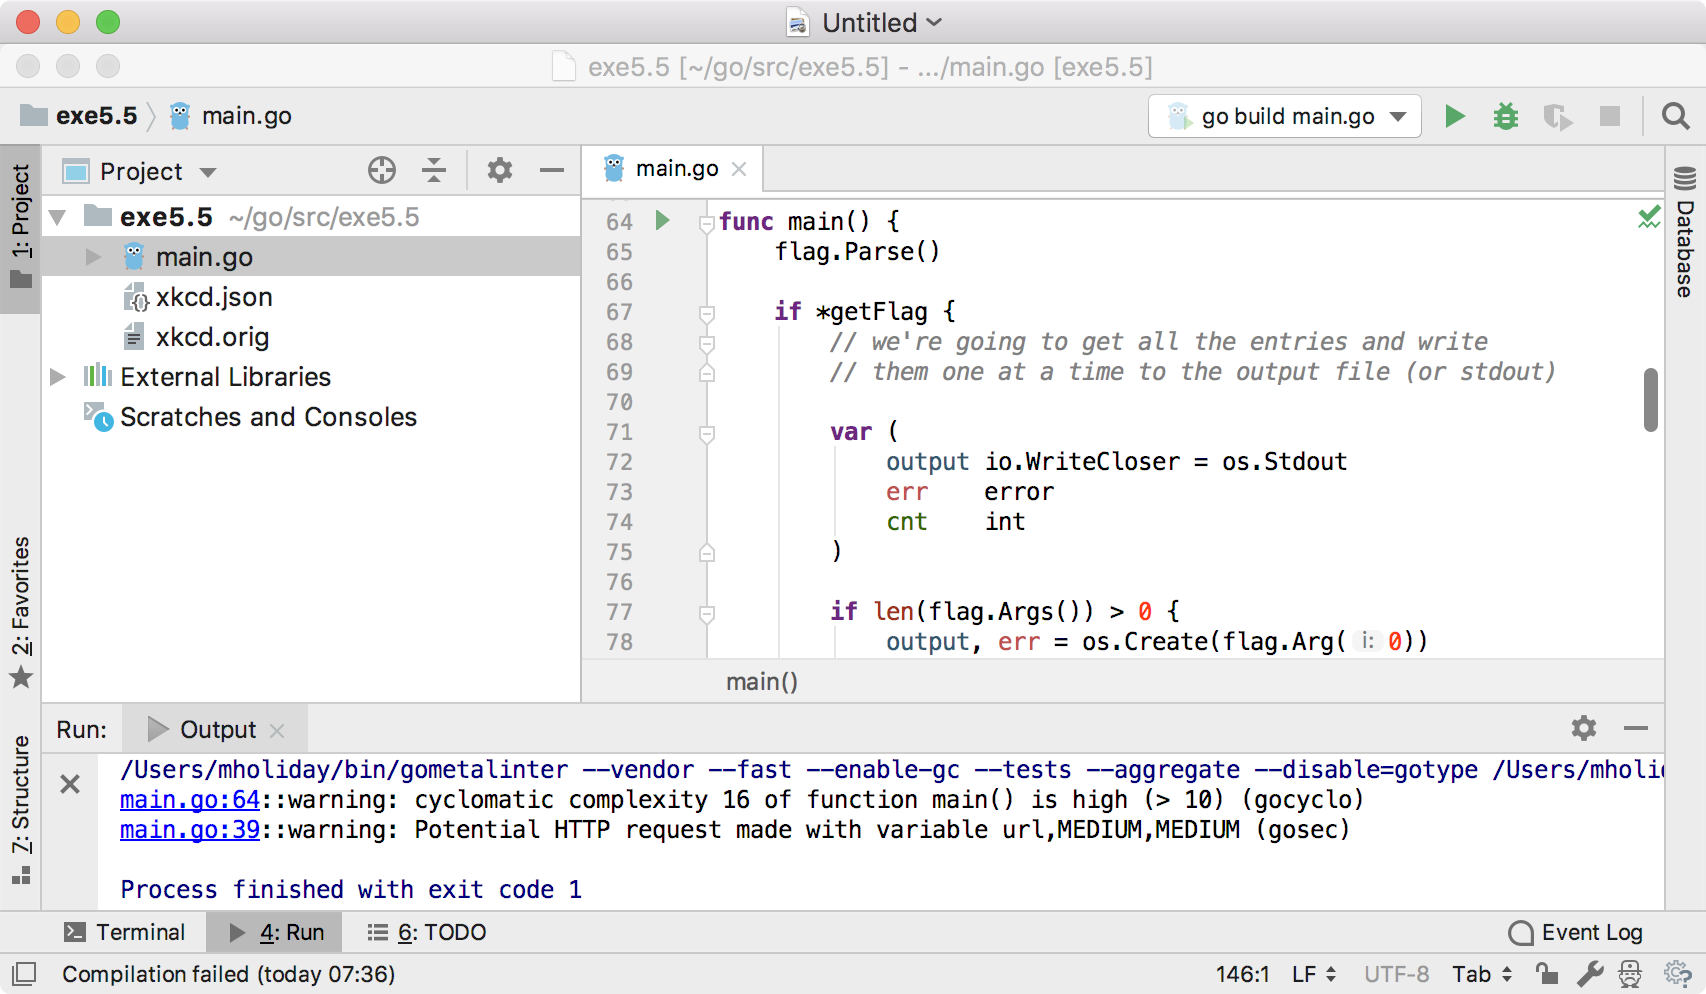
\includegraphics[width=\textwidth]{goland.png}
    \end{center}
\end{frame}

% =================================================================================

\section{Packages}
\begin{frame}[fragile]
\frametitle{Everything lives in a package}
Every standalone program has a \verb|main| package
\begin{golang}
package main

import "fmt"

func main() {
    fmt.Println("Hello, world!")
}
\end{golang}
\vspace{2\baselineskip}
Nothing is ``global''; it's either in your package or in another \par
\vspace{1\baselineskip}
It's either at  {\bf package} scope or {\bf function} scope
\end{frame}

\begin{frame}[fragile]
\frametitle{Packages control visibility}
Every name that's {\bf capitalized} is exported
\begin{golang}
package secrets

import . . .

type internal struct {
	. . .
}

func GetAll(space, name string) (map[string]string, error) {
	. . .
}
\end{golang}
\vspace{0.6\baselineskip}
That means another package in the program can import it \par
\vspace{0.4\baselineskip}
Within a package, {\em everything} is visible even across files
\end{frame}

\begin{frame}[fragile]
\frametitle{Package-level declarations}
You can declare anything at {\em package} scope
\begin{golang}
package secrets

const DefaultUUID = "00000000-0000-0000-0000-000000000000"

type k8secret struct {
    . . .
}

var secretKey string

func Do(it string) error {
   . . .
}
\end{golang}
\vspace{0.6\baselineskip}
But you can't use the short declaration operator \verb|:=| \par
\end{frame}

\begin{frame}[fragile]
\frametitle{Imports}
Each {\em source file} in your package must import what it needs
\begin{golang}
package secrets

import (
	"encoding/base64"
	"encoding/json"
	"fmt"
	"os"
	"strings"
)

. . .
\end{golang}
\vspace{0.6\baselineskip}
It may only import what it needs; unused imports are an error \par
\vspace{0.4\baselineskip}
Generally, files of the same package live together in a directory
\end{frame}

\begin{frame}[fragile]
\frametitle{What makes a good package?}
A package should embed deep functionality behind a simple API
\begin{golang}
package os

func Create(name string) (*File, error)
func Open(name string) (*File, error)

func (f *File) Read(b []byte) (n int, err error)
func (f *File) Write(b []byte) (n int, err error)
func (f *File) Close() error
\end{golang}
\vspace{2\baselineskip}
The Unix file API is perhaps the best example of this model \par
\vspace{0.5\baselineskip}
Roughly five functions hide a lot of complexity from the user
\end{frame}


\begin{frame}[fragile]
\frametitle{No cycles}
A package ``A'' cannot import a package that imports A
\begin{golang}
package A

import "B"

//------------------

package B

import "A"    // WRONG
\end{golang}
\vspace{1.5\baselineskip}
Move common dependencies to a third package \par
\vspace{0.5\baselineskip}
Or eliminate them \par
\end{frame}

\begin{frame}[fragile]
\frametitle{Initialization}
Items within a package get initialized before \verb|main|
\begin{golang}
const A = 1

var B int = C
var C int = A

func Do() error {
    . . .
}

func init() {
    . . .
}
\end{golang}
\vspace{\baselineskip}
Only the runtime can call \verb|init|, also before \verb|main|
\end{frame}

% =================================================================================

\section{Functions}
\begin{frame}[fragile]
    \frametitle{Functions in Go}
    Functions are ``first class'' objects; you can:
    \begin{itemize}
        \item Define them --- even inside another function
        \item Create anonymous {\em function literals}
        \item Pass them as function parameters / return values
        \item Store them in variables
        \item Store them in slices and maps (but not as keys)
        \item Store them as fields of a structure type
        \item Send and receive them in channels
        \item Write methods against a function type
        \item Compare a function var against \verb|nil|
    \end{itemize}
\end{frame}

\begin{frame}[fragile]
    \frametitle{Function scope}
    Almost anything can be defined inside a function
\begin{golang}
func Do() error {
    const a = 21

    type b struct {
        . . .
    }

    var c int

    func reallyDoIt() {
        . . .
    }
}
\end{golang}
\vspace{0.4\baselineskip}
{\em Methods} cannot be defined in a function (only at package scope)
\end{frame}

\begin{frame}[fragile]
    \frametitle{What is scope?}
    {\em Scope} is a term used to denote a region of the program \par
    \vspace{\baselineskip}
    It's the region of {\em visibility} of a name \par
    \vspace{\baselineskip}
    Scopes can be nested:
    \begin{itemize}
        \item Function within package
        \item Function within function
        \item Code block within function
    \end{itemize}
\end{frame}

\begin{frame}[fragile]
    \frametitle{Scope}
\begin{golang}
package xyz

var a int

func doIt() {
    var b int
    a = 2
    
    if b < 10 {
        a := 10
        . . .
    }
}
\end{golang}
Package-level \verb|a| can be seen inside \verb|doit|, but \verb|b| is {\em local} to \verb|doit| \par
\vspace{0.4\baselineskip}
There's another \verb|a| inside the \verb|if| block --- it {\em shadows} \verb|xyz.a|
\end{frame}

\begin{frame}[fragile]
    \frametitle{Scope vs lifetime}
    Scope is static, based on the code at compile time \par
\vspace{0.4\baselineskip}
    Lifetime depends on program execution
\begin{golang}
package xyz

func doIt() *int {
    var b int
    . . .
    
    return &b
}
\end{golang}
\vspace{0.4\baselineskip}
\verb|b| can only be seen inside \verb|doit|, but it will live past the return \par
\vspace{0.6\baselineskip}
It will live so long as part of the program keeps a pointer to it
\end{frame}

\begin{frame}[fragile]
    \frametitle{Shadowing short declarations}
    Short declarations with \verb|:=| have some gotchas \par
\begin{golang}
func main() {
	n, err := fmt.Println("Hello, playground")

	if _, err := fmt.Println(n); err != nil {
	    fmt.Println(err)
	}
}
\end{golang}
    \vspace{\baselineskip}
{\bf Compile error}: the first \verb|err| is unused \par
\vspace{0.6\baselineskip}
This follows from the scoping rules, because \verb|:=| is a declaration
and the second \verb|err| is in the scope of the \verb|if| statement
\end{frame}

\begin{frame}[fragile]
    \frametitle{Shadowing short declarations}
    Short declarations with \verb|:=| have some gotchas \par
\begin{golang}
func BadRead(f *os.File, buf []byte) error {
	var err error

	for {
		n, err := f.Read(buf) // shadows 'err' above

		if err != nil {
			break // causes return of wrong value
		}

		foo(buf)
	}

	return err // will always be nil
}
\end{golang}
\end{frame}


\begin{frame}[fragile]
    \frametitle{Function signatures}
    The {\em signature} of a function is the order \& type of its parameters\\
    and return values \par
    \vspace{0.5\baselineskip}
    It does not depend on the names of those parameters or returns \par
\begin{golang}
var try func(int, int) int

func Do(a, b int) int {
    . . .
}

func NotDo(x int, y int) a int {}
    . . .
}
\end{golang}
    \vspace{0.6\baselineskip}
These functions have the same {\em structural} type \par
\end{frame}

\begin{frame}[fragile]
    \frametitle{Structural typing}
    It's the same type if it has the same structure or behavior
\begin{golang}
type x func(int) int

func main() {
	var a x      // x is a named type

	b := func(y int) int {
		return y+2
	}

	a = b        // b is an anon func, but compatible
	fmt.Println(a(12))
}
\end{golang}
    \vspace{\baselineskip}
Go does use {\em structural} typing in most cases
\end{frame}

\begin{frame}[fragile]
    \frametitle{Structural typing}
    It's the same type if it has the same structure or behavior:
    \begin{itemize}
        \item arrays of the same size and base type
        \item slices with the same base type
        \item maps of the same key and value types
        \item structs with the same sequence of field names/types
        \item functions with the same parameter \& return types
    \end{itemize}
\end{frame}

\begin{frame}[fragile]
    \frametitle{Named typing}
    It's the only the same type if it has the same defined name
\begin{golang}
type x int

func main() {
	var a x      // x is a defined type; base int

	b := 12      // b defaults to int

	a = b        // TYPE MISMATCH

    a = 12       // OK, untyped literal
}
\end{golang}
    \vspace{\baselineskip}
Go does use {\em named} typing for non-function {\em defined} types
\end{frame}

\begin{frame}[fragile]
    \frametitle{Parameter passing}
    Parameters may be passed {\em by value} or {\em by reference}
\begin{golang}
func do(b []int) int {
	b[0] = 0
	b = []int{5, 6, 7}
	return b[2]
}

func main() {
	a := []int{1, 2, 3}
	v := do(a)

	fmt.Println(a, v)    // [0,2,3] 7
}
\end{golang}
\vspace{0.4\baselineskip}
``By value'' --- the parameter is copied into the function \par
\vspace{0.4\baselineskip}
``By reference'' --- the function can change the actual parameter
\end{frame}

\begin{frame}[fragile]
    \frametitle{Parameter passing}
    By value:
    \begin{itemize}
        \item numbers
        \item bool
        \item arrays
        \item structs
    \end{itemize}

    By reference:
    \begin{itemize}
        \item pointers to things, including structs
        \item strings (but they're immutable)
        \item slices (actually, a reference to the backing array)
        \item maps
        \item channels
    \end{itemize}
\end{frame}

\begin{frame}[fragile]
    \frametitle{Return values}
    Functions can have multiple return values
\begin{golang}
func doIt(a int, b []int) int {
    . . .

    return 1
}

func doItAgain(a string) (int, error) {
	. . .

    return 1, nil
}
\end{golang}
\vspace{\baselineskip}
Every return statement must have all the values specified
\end{frame}

\begin{frame}[fragile]
    \frametitle{Recursion}
    A function may call itself; the trick is knowing when to stop
\begin{golang}
func walk(node *tree.T) int {
    if node == nil {
        return 0
    }

    return node.value + walk(node.left) + walk(node.right)
}
\end{golang}
\vspace{2\baselineskip}
This works because each function call adds context to the stack\\
and unwinds it when done \par
\vspace{0.4\baselineskip}
If you don't have good stopping criteria, the program will crash
\end{frame}

% =================================================================================

\section{Closures}

\begin{frame}[fragile]
    \frametitle{What is a closure?}
    A {\em closure} is when a function inside another function ``closes over'' one or
    more local variables of the outer function \par
\begin{golang}
func fib() func() int {
	a, b := 0, 1

	return func() int {
		a, b = b, a+b
		return b
	}
}
\end{golang}
\vspace{0.4\baselineskip}
The inner function gets a {\bf reference} to the outer function's vars \par
\vspace{0.4\baselineskip}
Those variables may end up with a much longer {\em lifetime} than expected --- as
long as there's a reference to the inner function
\end{frame}

\begin{frame}[fragile]
    \frametitle{Closures: scope vs lifetime}
    The inner variables continue to live on \par
\begin{golang}
func fib() func() int {
	a, b := 0, 1

    // return a closure over a & b
}

func main() {
	f := fib()

    // f keeps ahold of a and b and updates them

	fmt.Println(f(), f(), f(), f(), f(), f())
}
\end{golang}
\vspace{0.4\baselineskip}
The inner function continues to mutate the variables it references
\end{frame}

\begin{frame}[fragile]
    \frametitle{Closure gotcha}
    Avoid closing over a variable that is mutating (a loop index)
\begin{golang}
func main() {
	s := make([]func(), 4)

	for i := 0; i < 4; i++ {
		s[i] = func() {
            // they all point to the same "i"
			fmt.Printf("%d %p\n", i, &i)
		}
	}

	for i := 0; i < 4; i++ {
		s[i]()
	}
}
\end{golang}
The program prints 4 each time; addresses all the same
\end{frame}

\begin{frame}[fragile]
    \frametitle{Closure gotcha}
    Avoid closing over a variable that is mutating (a loop index)
\begin{golang}
func main() {
	s := make([]func(), 4)

	for i := 0; i < 4; i++ {
		j := i // capture it before the closure
		s[i] = func() {
			fmt.Printf("%d %p\n", j, &j)
		}
	}

	for i := 0; i < 4; i++ {
		s[i]()
	}
}
\end{golang}
The program prints 1, 2, 3, 4 as expected; addresses different
\end{frame}

\begin{frame}[fragile]
    \frametitle{Closure gotcha}
    Avoid closing over a variable that is mutating (a loop index)
\begin{golang}
func main() {
	s := make([]func(), 4)

	for i := 0; i < 4; i++ {
		i := i // capture it before the closure
		s[i] = func() {
			fmt.Printf("%d %p\n", i, &i)
		}
	}

	for i := 0; i < 4; i++ {
		s[i]()
	}
}
\end{golang}
This does the same thing; one \verb|i| shadows the other
\end{frame}

% =================================================================================

\section{Defer}
\begin{frame}[fragile]
    \frametitle{Deferred execution}
    How do we make sure something gets done?
    \begin{itemize}
        \item close a file we opened
        \item close a socket / HTTP request we made
        \item unlock a mutex we locked
        \item make sure something gets saved before we're done
        \item ...
    \end{itemize}
\vspace{\baselineskip}
The \verb|defer| statement captures a function {\em call} to run later
\end{frame}

\begin{frame}[fragile]
    \frametitle{Defer}
    We need to ensure the file closes no matter what
\begin{golang}
func main() {
	f, err := os.Open("my_file.txt")

    if err != nil {
        . . .
    }

    defer f.Close()

    // and do something with the file
}
\end{golang}
\vspace{0.6\baselineskip}
The call to \verb|Close| is guaranteed to run at function exit \par
\vspace{0.4\baselineskip}
Don't defer closing the file until we know it really opened
\end{frame}

\begin{frame}[fragile]
    \frametitle{Defer gotcha \#1}
    The scope of a \verb|defer| statement is the {\em function}
\begin{golang}
func main() {
    for i := 1; i < len(os.Args); i++ {
	    f, err := os.Open(os.Arg(i))
    
        . . .

        defer f.Close()

        . . .
    }
}
\end{golang}
\vspace{0.6\baselineskip}
The deferred calls to \verb|Close| must wait until function exit \par
\vspace{0.4\baselineskip}
We might run out of file descriptors before that!
\end{frame}

\begin{frame}[fragile]
    \frametitle{Defer gotcha \#2}
    Unlike a closure, \verb|defer| copies arguments to the deferred call
\begin{golang}
func main() {
	a := 10

	defer fmt.Println(a)

	a = 11

	fmt.Println(a)
}

// prints 11, 10
\end{golang}
\vspace{0.6\baselineskip}
The parameter \verb|a| gets copied at the \verb|defer| statement \par
\vspace{0.4\baselineskip}
The \verb|defer| statement doesn't get a reference
\end{frame}

\begin{frame}[fragile]
    \frametitle{Defer gotcha \#2}
    A \verb|defer| statement runs before the \verb|return| is done
\begin{golang}
func doIt() (a int) {
	defer func() {
        a = 2
    }()

	a = 1
    return
}

// returns 2
\end{golang}
\vspace{0.6\baselineskip}
We have a named return value and a ``naked'' return \par
\vspace{0.4\baselineskip}
The deferred anonymous function can update that variable
\end{frame}

% =================================================================================

\section{Homework}
\begin{frame}[fragile]
    \frametitle{Homework \#2}
    Exercise 5.5 from {\em GOPL:} implement \verb|countWordsAndImages| \par
    \vspace{\baselineskip}
    Actually, given some HTML as raw text, parse it into a document and
    then call your counting routine to detect and count words and images
    (you can follow the book's example). \par
    \vspace{\baselineskip}
    Don't worry about getting HTML from an HTTP query; we're not there yet. \par
    \vspace{\baselineskip}
    See Homework \#1 for counting words. \par
    \vspace{\baselineskip}
    What happens if the HTML document is empty? \par
\end{frame}

% \begin{frame}[fragile]
% \frametitle{Homework \# 2}
% Example input:
% \begin{golang}
% var raw = `
% <!DOCTYPE html>
% <html>
%   <body>
%     <h1>My First Heading</h1>
%       <p>My first paragraph.</p>
%       <p>HTML images are defined with the img tag:</p>
%       <img src="xxx.jpg" width="104" height="142">
%   </body>
% </html>`
% \end{golang}
% \end{frame}

\end{document}
